
Up until this point, the focus was mainly on the single scores, mostly from the same type and method, to improve the separation between the scores of the \ac{MSA} superfamily and the others. The following section analyzes the reverse-corrected scores and the simple-corrected scores from the same method together.
 

Figure \ref{fig:scatter} shows scatterplots with the simple-corrected scores on the horizontal axis and the reverse-corrected scores on the vertical axis, generated from the original score with the primary structure only on top, and including the secondary structure information below. For both approaches, Viterbi and forward scoring, the improvements using the secondary structure are obvious, as the separation between the superfamily scores and the others increases. 
However, this result was already expected based on the figures provided in this section. The same plot for all other variations of the \ac{MSA} \texttt{c.67.1} shown in this section can be found in Appendix \ref{app:APPPCAcorrScores}. 


\begin{figure}[H]
	\begin{center}
		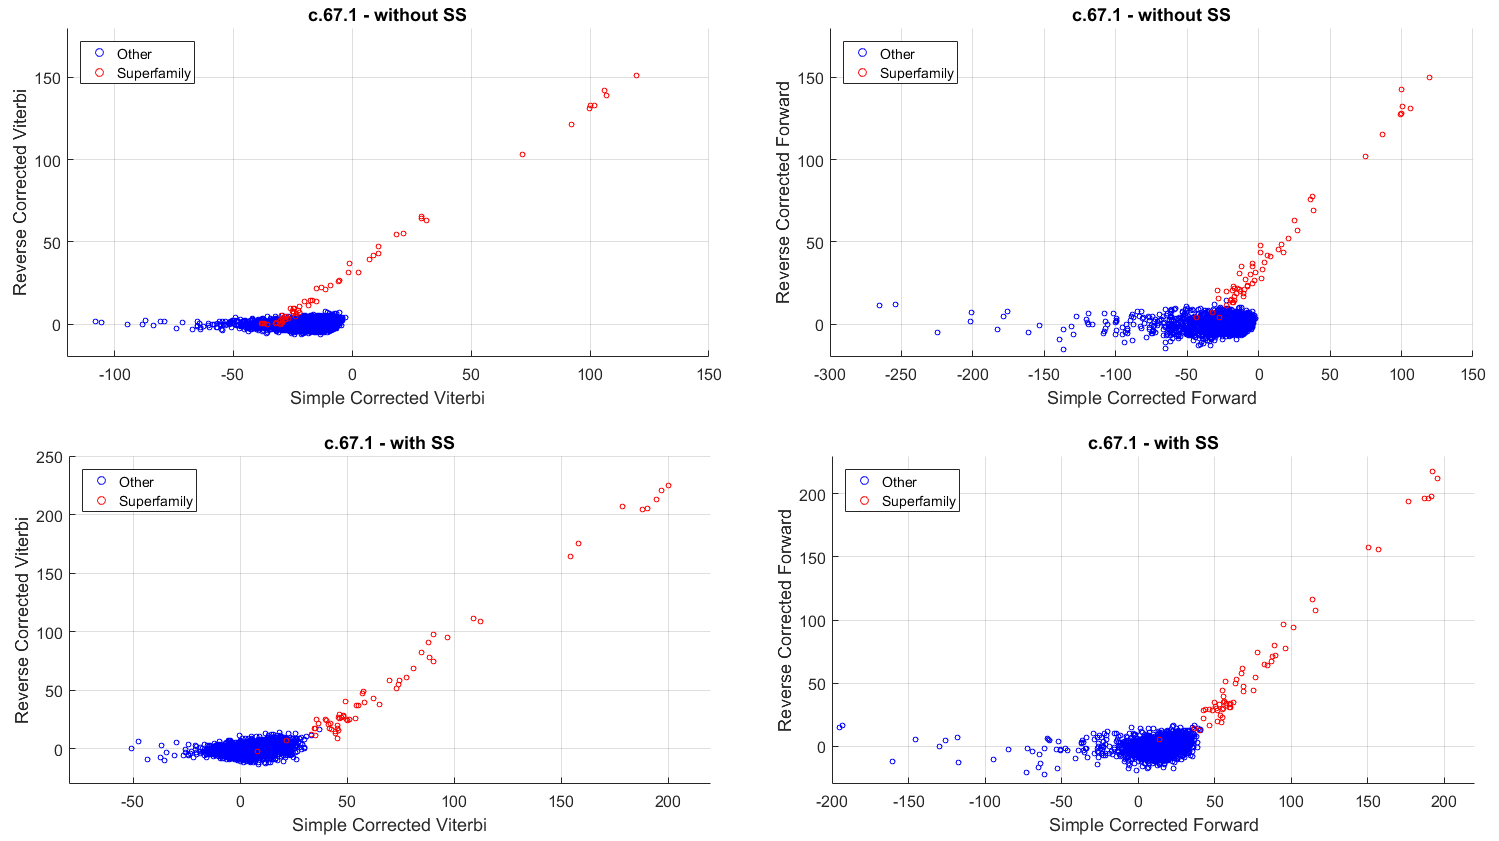
\includegraphics[width=\textwidth]{fig/scatter}
	\end{center}
	\caption{Scatterplots of the corrected scores with and without secondary structure information.}	
	\label{fig:scatter}
\end{figure}

This two-dimensional representation with its variety of post-processing methods is used in the following section for the evaluation of all 69 \acp{MSA} with varying weighting methods.


\section{Evaluation of the Different Weighting Methods}
\label{sec:weightingMeth}

The different weighting methods and their parameters described in  Section \ref{sec:training} will be tested by scoring all 69 \acp{MSA} against the \ac{SCOP} database with different settings. The following five configurations will be explained in more detail.

\begin{itemize}
\item \texttt{M1\_025\_1} uses the weighting approach in (\ref{eq:mix1}), with a pseudo-count of 1 for the secondary structure emission probabilities and a threshold of 0.25 for the highest primary structure emission probability. 

\item \texttt{M1\_025\_3} uses the same approach as above, except with a pseudo-count of 3.

\item \texttt{M2\_025\_1\_3} uses the weighting approach in (\ref{eq:mix2}), also with a threshold of 0.25 and a pseudo-count of 1. The scale factor $k$ is set to 3. 

\item \texttt{M2\_025\_1\_5} uses the same parameters as M2\_025\_1\_3 except with a scaling factor of 5.

\item \texttt{M3\_100\_5} uses the Shannon approach in (\ref{eq:shannonfinal}) with a pseudo-count of 5 for generating the secondary structure emission probabilities. A threshold of 100\,\% is also employed, resulting in only the mixed probabilities being used for scoring.
\end{itemize}

For example, with the \ac{MSA} \texttt{c.67.1}, the threshold of 0.25 for the first four approaches results in 272 columns where the highest emission probability is below the threshold; therefore, the mixed probabilities are used, containing both the primary and the secondary structure. For the other 117 columns of the \ac{pHMM}, only the emission probabilities for the primary structure are used. For the last method, using the Shannon entropy, it was found that the best results are achieved using the mixed probabilities only.

The different methods over the \acp{MSA} are compared in MATLAB as listed in \ref{LST_svmMat} by generating a \ac{ROC} curve. A \ac{ROC} curve compares the \ac{TPR} against the \ac{FPR} for varying thresholds of a classifier and is used to compare the quality of classifiers. The \ac{TPR} measures the proportion of positives that are correctly classified as such, while the \ac{FPR} identifies negatives that are wrongly classified as positives (see \cite[p. 34--35]{Duda.2001}).

\lstset{
keywords={fitcsvm, fitPosterior, resubPredict, perfcurve},numbers=left, captionpos=b,	tabsize=4, numbersep=10pt, commentstyle=\color{dkgreen}, keywordstyle=\color{blue},
	showspaces=false, 
basicstyle  = \fontfamily{pcr} \fontsize{9pt}{10pt} \selectfont \singlespacing ,}
\begin{lstlisting}[caption=Matlab implementation for generating the \ac{ROC} curve. ,
label=LST_svmMat]
mdlSVM = fitcsvm(hmmScores,classes,'Standardize',true);
mdlSVM = fitPosterior(mdlSVM);
[~,score_svm] = resubPredict(mdlSVM);
[X,Y,T,AUC] = perfcurve(hmmScores,score_svm(:,mdlSVM.ClassNames),'true');
plot(X,Y)
\end{lstlisting}

 For each method and \ac{MSA}, the function \textit{fitcsvm} trains a binary \ac{SVM} classifier from \textit{hmmScores}, containing the two dimensions for the reverse-corrected and the simple-corrected scores and the \textit{classes}, indicating whether the score relates to the tested superfamily or not. The function \textit{fitPosterior} calculates the posterior probabilities for all scores, allowing \textit{perfcurve} to generate the \ac{ROC} curve.



Figure \ref{fig:roc} shows the \ac{ROC} curve generated for the superfamily \texttt{c.67.1} using the methods described above, as well as the original score using only the primary structure listed as \textit{AA}. The scores used are the two corrected Viterbi scores, with the \mbox{reverse-corrected} Viterbi as the first principal component from the score with and without secondary structure information.
The six scatterplots used for this \ac{ROC} plot are shown in Appendix \ref{app:APPPCAcorrScoresWeight}.
As an optimal classifier would be a rectangular graph with 100\% \ac{TPR}  at 0\% \ac{FPR}, the improvement of the new methods using secondary structure information is obvious.

\begin{figure}[H]
	\begin{center}
		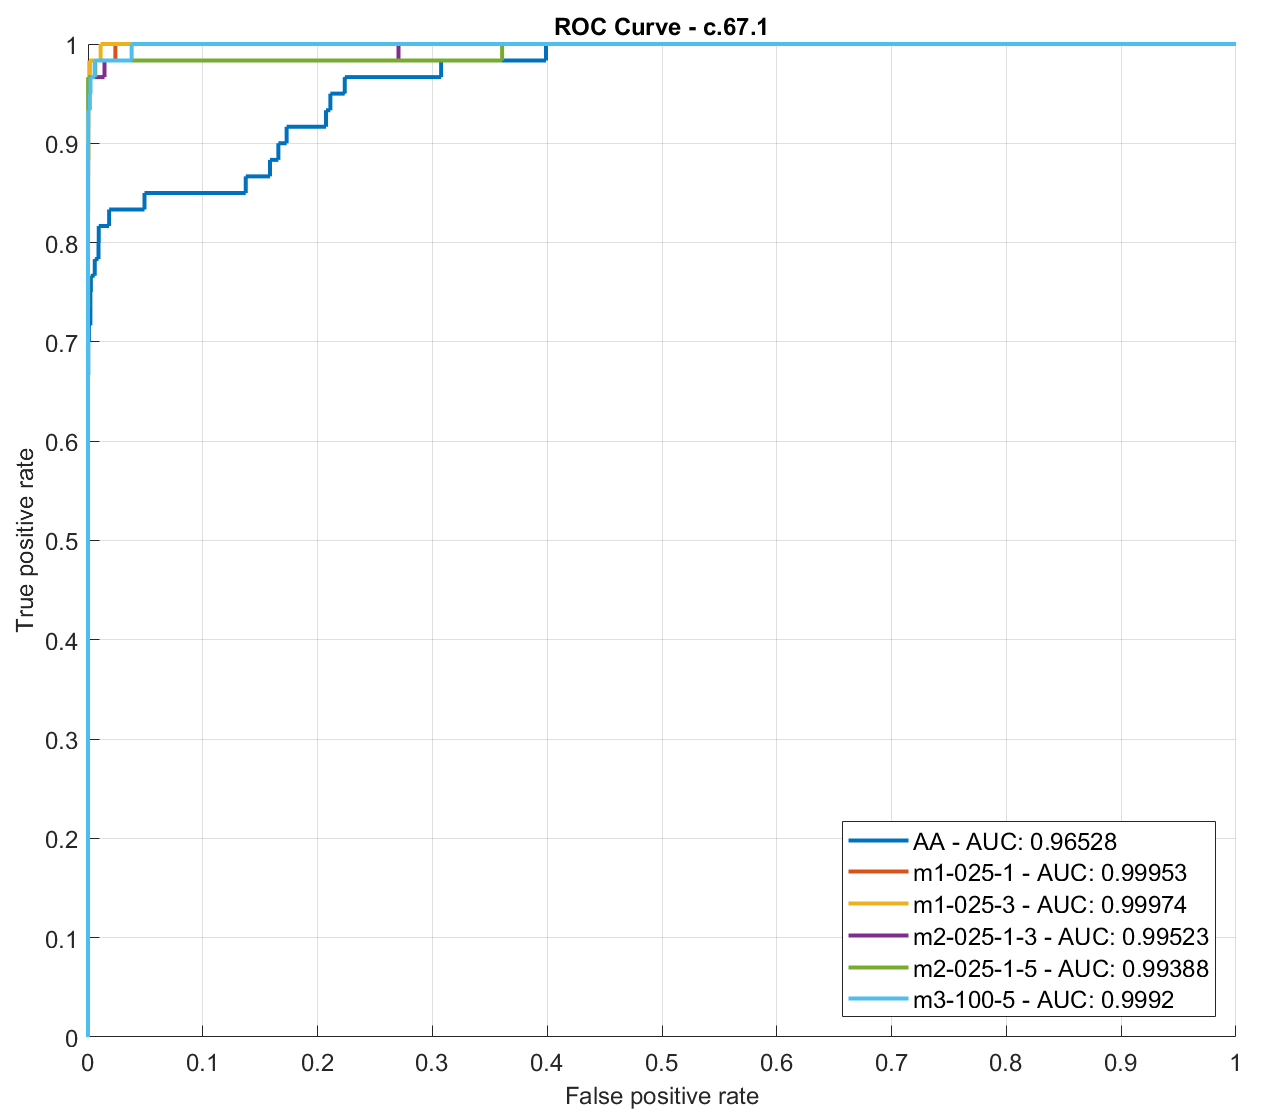
\includegraphics[width=0.8\textwidth]{fig/roc}
	\end{center}
	\caption{\acs{ROC} curve for the \acs{MSA} c.67.1.}
	\label{fig:roc}
\end{figure}

For comparison of the different methods, the \ac{ROC} curves can be ranked with the \ac{AUC} score. The \ac{AUC} score combines the whole \ac{ROC} curve into one number in the range of 0--1 and is calculated by the integral of the curve. 

Table \ref{tab:ROC} provides an overview of the selected methods for the \ac{MSA}. However, the table lists only 56 \acp{MSA}, as those with  a variation of the AUC score below 1\% were filtered out. Column \textit{AA} lists the \ac{AUC} score using only the primary structure. The highest \ac{AUC} score for each \ac{MSA} is highlighted in green, while all scores below those obtained using the original method  are highlighted in red. To summarize the table, it can be said that except for a few scores, the secondary structure information improves the quality of the homology detection. For all \acp{MSA}, the original score was improved by at least one method including the secondary structure. The best results were achieved with the method \texttt{M2\_025\_1\_5}, with only two scores below the original score and 29 with the highest rank. 


The \ac{AUC} scores for all \acp{MSA} were also compared to the different corrected scores and their combinations discussed in Section \ref{ssec:Scores_Changes}. 
The results are summarized in Table \ref{tab:ovAllAUC}, with the first number of each cell providing the number of scores above those of the original method using only the primary structure. The second number counts the \acs{MSA} with the highest \ac{AUC} scores compared to all other methods. The table shows that the method \texttt{M2\_025\_1\_5} performed best for the most score types, compared to the other methods. The best score type varies across the different methods. For the highest-ranked method, the Viterbi method performs better than the old method for 65 of 69 scores.  However, over all methods, both \ac{PCA} variations for the Viterbi yield a larger improvement than the plain scores. The last column represents the combination of the Viterbi and forward scores. 
In general, this score type performs worse than the other types, with seven \acp{MSA} where the original method has higher scores than all methods that use the secondary structure information.


\definecolor{Gray}{gray}{0.9}
\newcolumntype{g}{>{\columncolor{Gray}}r}
\newcolumntype{h}{>{\columncolor{Gray}}l}
\begin{table}[h!]
\centering
\begin{tabular}{|l|g:h|r:l|g:h|r:l|g:h|}
         \hline
 \multirow{2}{*}{\backslashbox{\small{Method}}{\small{Score-type}}}      & \multicolumn{10}{c|}{ \# scores with AUC > AA ; \# highest scores for method } \\
              & \multicolumn{2}{c|}{Viterbi}                       & \multicolumn{2}{c|}{Forward} & \multicolumn{2}{c|}{PCA-Vit.} & \multicolumn{2}{c|}{PCA-For.} & \multicolumn{2}{c|}{PCA-VitFor} \\ \hline
AA     		  & 					  			&  \: 1 			   & 			 & \: 1      			&               & \: 2          &               &  \: 2    			       	&                  & \: 7  \\ \hline
M1\_025\_1    & 55                    			& 13                   & 54          & 12         			& 60            & \: 8          & 62            & 12     			        & 55              & 11             \\ \hline
M1\_025\_3    & 57                    			& 16                   & 56          & 16         			& 59            & 16            & 63            & 11       					& 51              & 13             \\ \hline
M2\_025\_1\_3 & 49                    			& \: 4                 & 50          & \: 4         		& 54            & \: 4          & 58            & \: 2    			        & 53              & \: 5              \\ \hline
M2\_025\_1\_5 & 65                    			& 28                   & 64          & 28         			& 64            & 33            & 62            & 29       					& 56              & 27             \\ \hline
M3\_100\_5    & \quad 55             			& \: 7            & \quad 46         & \: 8          		& \quad 54      & \: 6            & \quad 59      & 13             & \: \: 55              & \: 6        \\  \hline
\end{tabular}
	\caption[Performance of different scoring methods.]{Performance of different scoring methods for the corrected scores over all 69 \acsp{MSA}. First column lists number of \acs{AUC} scores above the score using primary structure only (AA), second column number of highest scores for the method. }
	\label{tab:ovAllAUC}

\end{table}

The \ac{AUC} scores for each score type and the method of all 69 \acp{MSA} represented in Table \ref{tab:ovAllAUC}, including their associated scatterplots and ROC curves, can be found on the attached disk (see Appendix \ref{app:AppDisk}).




\def\g{\cellcolor{green!25}}
\def\r{\cellcolor{red!25}}
\def\y{\cellcolor{yellow!10}}

% Please add the following required packages to your document preamble:
% \usepackage{graphicx}
\begin{table}[H]
\centering
\resizebox{\textwidth *6/7}{!}{%
 \renewcommand{\arraystretch}{0.8}
\begin{tabular}{|l|c|ccccc|}
\hline
MSA      &  AA  \qquad & M1\_025\_1 & M1\_025\_3 & M2\_025\_1\_3 & M2\_025\_1\_5 & M3\_100\_5 \\ \hline
a.1.1   & \enskip \y 0.981660 \enskip & \enskip \g 0.999138 \enskip   &  \enskip 0.998953 \enskip  & \enskip 0.992644 \enskip     & \enskip 0.997789 \enskip     &  \enskip 0.997729 \enskip   \\ 
a.118.1 & \y 0.658467      & 0.753259      & 0.705426      & 0.746597      & \g 0.829309      & \r 0.644325       \\
a.118.8 & \y 0.955319      & 0.984794      & 0.985946      & \g 0.986001      & 0.973027      & 0.977922       \\
a.121.1 & \y 0.949624      & 0.995763      & 0.995620      & 0.996995      & \g 0.997438      & 0.983587       \\
a.25.1  & \y 0.841495      & 0.937005      & 0.932636      & 0.941242      & \g 0.957592      & 0.937555       \\ \hline
a.26.1  & \y 0.874773      & 0.983614      & 0.985165      & 0.969996      & \g 0.985939      & 0.964079       \\
a.39.1  & \y 0.952474      & 0.981174      &  \g 0.982275      & 0.959055      & 0.979119      & \r 0.948074       \\
a.4.1   & \y 0.943772      & 0.955631      & 0.952669      & \g 0.969677      & 0.964489      & \r 0.918509       \\
a.4.5   & \y 0.855347      & 0.926701      & 0.925346      & 0.908423      & \g 0.929703      & 0.916538       \\
b.1.18  & \y 0.792153      & 0.817158      & 0.807228      & 0.815886      & \g 0.838580      & 0.802668       \\  \hline
b.1.2   & \y 0.969961      & 0.995894      & 0.995995      & 0.981565      & 0.993793      & \g 0.997065       \\
b.121.4 & \y 0.773631      & 0.967558      & 0.966382      & 0.866694      & \g 0.992417      & 0.953065       \\
b.122.1 & \y 0.848138      &  \r 0.845888      &  \r 0.848104      & \r 0.845576      & \g 0.851568      &  \r 0.779088       \\
b.18.1  & \y 0.761240      & 0.930075      &  \g 0.936217      & 0.817446      & 0.866923      & 0.929797       \\
b.29.1  & \y 0.696135      & 0.960836      & 0.951235      & 0.849526      & \g 0.983435      & 0.940170       \\  \hline
b.40.4  & \y 0.562231      & 0.645208      &  \g 0.670961      & 0.569530      & \r 0.338704      & 0.567449       \\
b.55.1  & \y 0.911226      & 0.979285      &  \g 0.980650      & 0.929043      & 0.959400      & 0.957248       \\
b.6.1   & \y 0.908563      & 0.960190      &  \g 0.966697      & 0.937017      & 0.955984      & 0.957871       \\
b.60.1  & \y 0.930032      & 0.984104      & 0.984354      & 0.970134      & \g 0.990348      & 0.978497       \\
b.82.1  & \y 0.825039      & 0.938847      & 0.919836      & 0.866187      & \g 0.955784      & 0.912106       \\  \hline
c.1.10  & \y 0.873501      & 0.874392      &  \r 0.869691      & \r 0.872736      & \g 0.940628      & \r 0.872383       \\
c.1.8   & \y 0.771208      & 0.928533      & 0.936710      & 0.773840      & 0.930788      & \g 0.945124       \\
c.1.9   & \y 0.776061      & 0.984452      &  \g 0.987866      & 0.849393      & 0.953804      & 0.968378       \\
c.14.1  & \y 0.922587      & 0.973523      &  \g 0.978553      & \r 0.895175      & 0.937373      & 0.943083       \\
c.2.1   & \y 0.832922      & 0.877780      &  \g 0.878903      & \r 0.830230      & 0.874660      & 0.849042       \\  \hline
c.23.16 & \y 0.953418      & 0.984812      &  \g 0.985526      & \r 0.946543      & 0.970777      & 0.979098       \\
c.23.1  & \y 0.982697      & 0.997496      & 0.996486      & 0.996668      & \g 0.998236      & 0.994347       \\
c.26.1  & \y 0.948562      & 0.976231      &  \g 0.976961      & 0.960769      & 0.965366      & 0.976797       \\
c.26.2  & \y 0.762557      & 0.851986      & 0.846154      & 0.772628      & \g 0.903711      & 0.878560       \\
c.3.1   & \y 0.873175      & 0.889874      & 0.884938      & 0.874126      & \g 0.900207      & \r 0.855220       \\  \hline
c.37.1  & \y 0.566633      & 0.757238      & 0.705066      & 0.633610      & \g 0.795116      & 0.721068       \\
c.47.1  & \y 0.758197      & 0.851974      & 0.840546      & 0.832753      & \g 0.889316      & 0.819158       \\
c.52.1  & \y 0.715274      &  \r 0.687236      &  \r 0.689456      & 0.728182      & \g 0.729141      & \r 0.689634       \\
c.55.1  & \y 0.841824      & 0.890524      & 0.888006      & 0.872482      & 0.879920      & \g 0.896231       \\
c.55.3  & \y 0.661511      & 0.724718      & 0.730029      & 0.745105      & \g 0.827794      & 0.708841       \\  \hline
c.56.5  & \y 0.932965      & 0.975813      & 0.976139      & \r 0.931557      & \g 0.988531      & 0.970057       \\
c.66.1  & \y 0.691936      & 0.792645      & 0.805687      & 0.762319      & \g 0.828899      & 0.826029       \\
c.67.1  & \y 0.965279      & 0.999527      &  \g 0.999741      & 0.995230      & 0.993875      & 0.999198       \\
c.68.1  & \y 0.840345      & 0.954689      &  \g 0.955924      & 0.896832      & 0.953844      & 0.942945       \\
c.69.1  & \y 0.769510      & 0.951119      &  \g 0.954956      & 0.886774      & 0.945654      & 0.938550       \\  \hline
c.94.1  & \y 0.786186      & 0.885272      & 0.891178      & 0.822143      & \g 0.910847      & 0.838724       \\
d.108.1 & \y 0.842174      &  \g 0.985350      & 0.985037      & 0.890825      & 0.959523      & 0.956787       \\
d.129.3 & \y 0.770835      & 0.906587      & 0.886342      & 0.779503      & 0.887589      & \g 0.929245       \\
d.14.1  & \y 0.800006      & 0.820208      & 0.828362      & 0.813035      & \g 0.884108      & 0.847360       \\
d.144.1 & \y 0.970321      & 0.980958      &  \r 0.968978      & \r 0.968810      & \g 0.985398      & 0.979926       \\  \hline
d.15.1  & \y 0.820850      & 0.841835      & 0.836335      & 0.938895      & \g 0.945733      & \r 0.819833       \\
d.153.1 & \y 0.904484      & 0.963783      &  \g 0.964523      & 0.911143      & 0.941617      & 0.949000       \\
d.169.1 & \y 0.914845      & 0.984051      & 0.986197      & 0.949123      & \g 0.987850      & 0.936318       \\
d.17.4  & \y 0.917448      &  \g 0.997716      & 0.997654      & 0.949466      & 0.988231      & 0.996560       \\
d.3.1   & \y 0.781971      &  \g 0.922795      & 0.913319      & 0.795755      & 0.889231      & 0.920976       \\  \hline
d.32.1  & \y 0.943212      & 0.988796      &  \g 0.991518      & 0.974388      & 0.983423      & 0.983284       \\
d.38.1  & \y 0.927538      & 0.975661      & 0.971830      & 0.955195      & \g 0.986411      & 0.971640       \\
d.58.4  & \y 0.923971      & 0.939588      & 0.928788      & 0.936421      & \g 0.951176      & 0.935353       \\
d.81.1  & \y 0.803026      & 0.821645      & 0.809742      & \r 0.798986      & 0.823577      & \g 0.824889       \\
d.92.1  & \y 0.747920      & 0.791525      & 0.794027      & 0.803735      & \g 0.833569      & 0.819230       \\  \hline
g.39.1  & \y 0.984596      & \r 0.982231      & \r 0.982742      & \g 0.988259      & \r 0.983898      & \r 0.976715  \\ \hline
\end{tabular}%
}
\caption[\acs{AUC} scores for the different scoring methods.]{\acs{AUC} scores for the different scoring methods from the corrected Viterbi scores postprocessed with \acs{PCA} compared to the original method in column AA using primary structure only. The highest score for each \acs{MSA} is marked green. Red scores are below the original method.   }
\label{tab:ROC}
\end{table}



